\documentclass[tcc]{subfiles}

\begin{document}

\chapter{Results and discussion}
\label{sec:results}
\epigraph{Que tanto de peça para dar defeito.\\{\footnotesize (That's a lot of parts to malfunction.)}}{- My grandfather about my father's new car}

\section{Engine matching}
\begin{sidewaysfigure}[p]
    \AddThispageHook{\thispagestyle{empty}}
    \caption{Component maps and work line of the VT-80 engine}
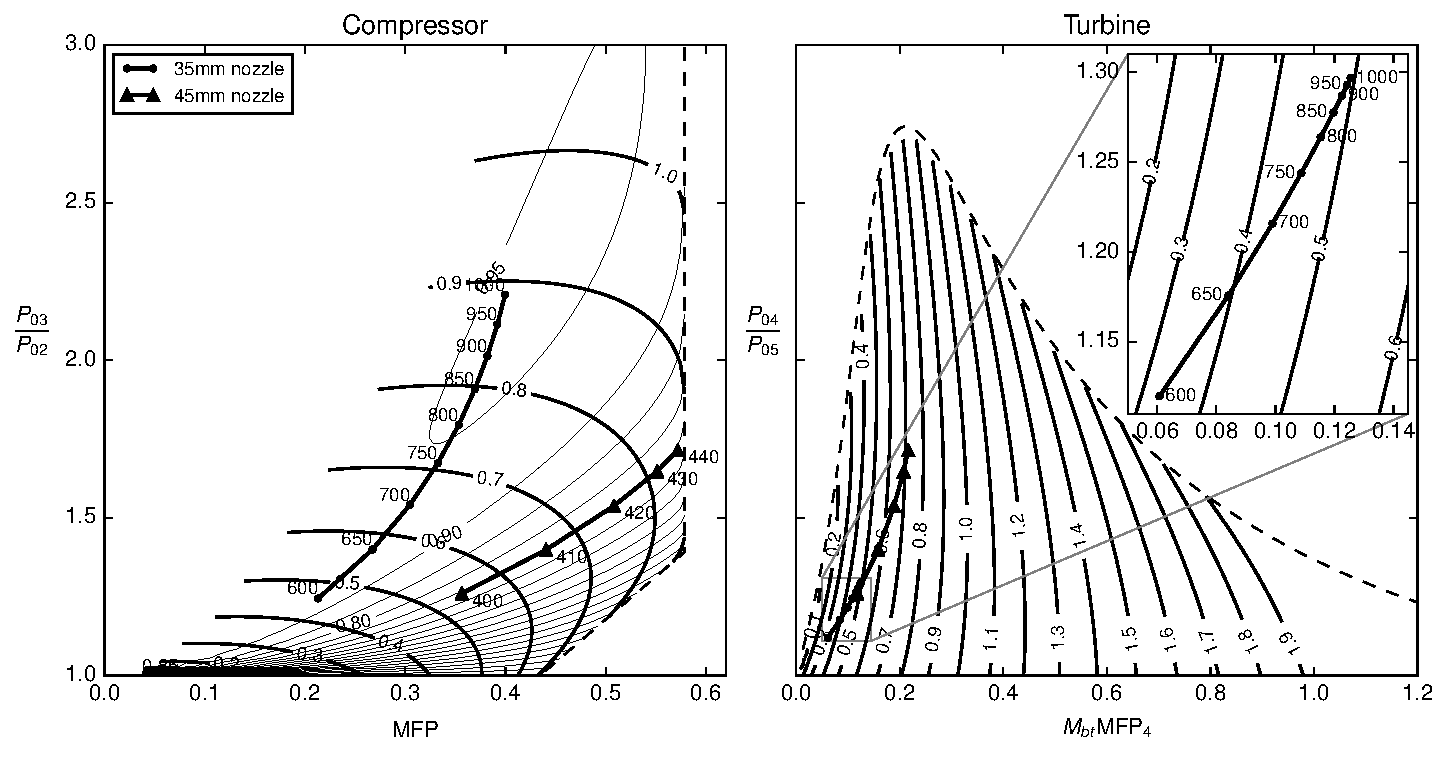
\includegraphics{fig/wline.pdf}
    \source{author's figure}
    \legend{Compressor and turbine maps for the VT-80 engine, with the work line superimposed (thick line).
    The medium thickness contours are of constant blade mach number and the thin contours are of constant polytropic efficiency.}
\end{sidewaysfigure}

\begin{figure}
    \caption{Flow state at each engine station}
    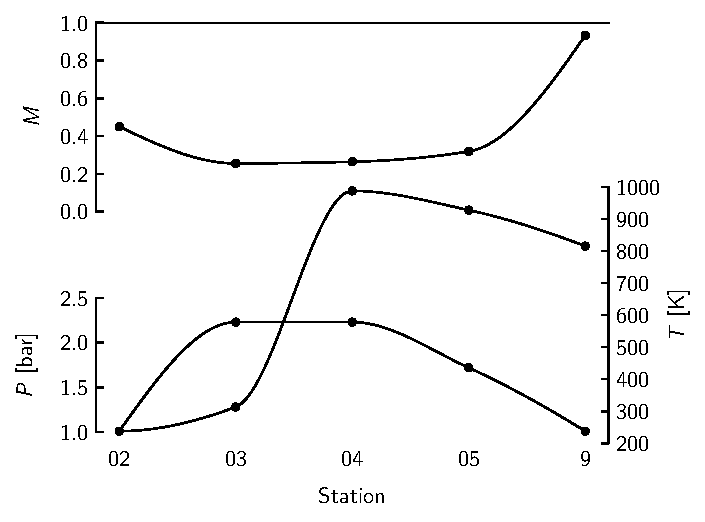
\includegraphics{fig/stations1000K}
    \source{author's figure}
    \caption*{Temperature, pressure and mach number for each engine station at a turbine inlet temperature of 1000K and flight mach number zero. The temperature and pressure scales were chosen to keep their ratios to the reference values $\mathsf P_{01}$ and $\mathsf T_{01}$ comparable. When the station number is prefixed with a ``0'', the properties are from stagnation, otherwise they are static. Interpolation was done with the PCHIP algorithm \cite{Fritsch1980}, to keep lines smooth while not introducing artificial maxima.}
\end{figure}

Compressor and turbine show a nice match, even though many of the losses are not included in the model.
This is probably due to the overly optimistic efficiencies in both the compressor and the turbine compensating for each other.

turbine has a poor design because it tends to choke on exit instead of on inlet.

nozzle seems to be too big for the engine. In the simulation it was reduced from the measured diameter of 45mm to 35mm. This may be due to the overestimation of the components' efficiencies.

\todo{parameters used for simulation}

\begin{figure}
    \caption{Matching sensitivity to nozzle diameter}
\end{figure}

\section{Dynamical simulation}

\end{document}
